


\chapter{Hardware}
\label{chap:Hardware}

\section{Hardware Components}
\label{sec:intro}
The previous hardware was setup by Mr. Pravin Dhake in  \cite{dhake2007real}  and Mr. Robert Woodley \cite{woodley1999testbed}. In their work, Woodley and Dhake put together a trailer truck with control and data acquisition libraries. This trailer truck has the ability to move automatically with the position given to it. In the course of this project the same truck is used but with updated components and libraries are developed to perform 3D modeling. Table \ref{table:Hardware} tabulates all the hardware used in the system.


\begin{table}[ht]
 \centering
  \caption{Overview of all the Hardware on the Truck }
 \begin{tabular}{||c|c||}
 \hline \hline
  $\vspace{0.02in} \textbf{Name of the Part}$ & $\vspace{0.02in} \textbf{Description}$ \\
 \hline \hline
  Controller Board  & AAEON PFM-945C \\
 \hline
 Frame Grabber  & Sensoray model 911 \\
 \hline
Storage for controller board    & SSD-104 SATA \\
\hline
PCI-104 to PC-104 converter     & Connect Tech PCI-104 to PC-104 Adapter \\ 
\hline
A to D Converter    & AIM Multi-IO 104 \\
\hline
Motor controller board & Mesa Electronics 4I27 Motor controller \\ 
\hline
Accelerometer   & Dimension Engineering ACCM3D \\
\hline
Steering Motor  & Futuba FP-S148  \\
\hline
Driver Motor    & RS-550 DC permanent magnet motor  \\
\hline
Potentiometer   & Bourns Potentiometer  \\
\hline\hline
 \end{tabular}

    \label{table:Hardware}
\end{table}





\subsection{Controller Board-AAEON PFM-945c}
It is a low power PC-104 form factor based board, that is very suitable for our application because of its atom processor and its form factor, more details about the board are given in \cite{Aaeon}. The board is supposed to run a real time operating system and should do both the image processing and the motion control functions. The board needs a 12V @1.5A power supply to function and is capable of handling both PCI-104 and PCI-express buses. This is an upgrade over the GX533 board which was used as part of Dhake's work in \cite{dhake2007real}. This board is powered by an atom processor by Intel and is capable of running both Linux and Windows. Through extensive testing, it was found that the board runs very well with a stripped down version of Ubuntu 12.04. Figure \ref{fig:specs1} shows a picture of the board, and Table \ref{table:Controller} lists the basic specifications of the board. 
\begin{figure}[ht]
    \centering
    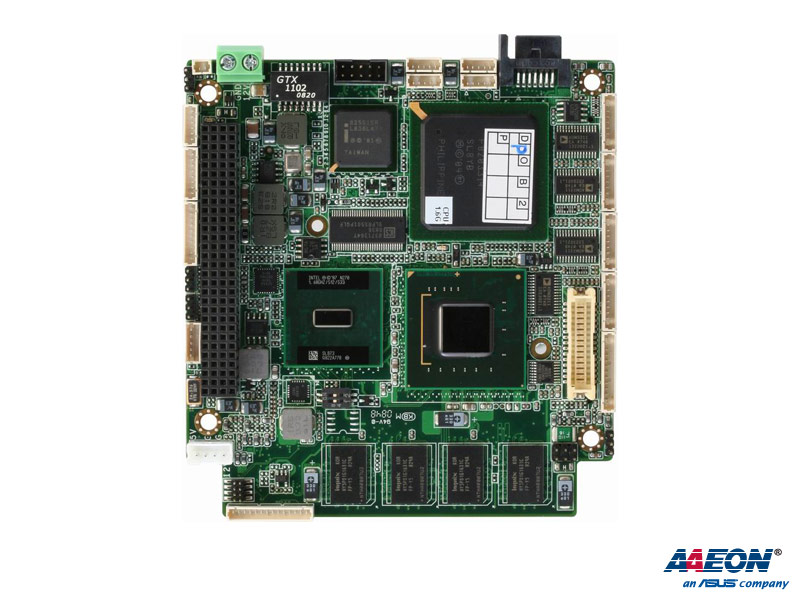
\includegraphics[width=10cm,height=10cm,keepaspectratio]{Pictures/controller.jpg}
    \caption{Controller\label{fig:specs1}} 
\end{figure}


\begin {table}[ht]
 \centering
\caption{Controller}
 \begin{tabular}{||c|c||}
 \hline \hline
  Processor   & Onboard Intel Atom N270 1.6 GHz Processor \\
 \hline
  Memory & Onboard DDR2 400/533 Memory 512 MB/ 1 GB \\
 \hline 
  Chipset & Intel 945 GSE \\
  \hline
  Communication Interface & PCI-104 Express (PCI-104 + PCI-104e) \\
  \hline
  Board Size  & 4.05" (L) x 3.77" (W) (102.8mm x 96mm) \\
  \hline
  Power Requirement & 1.56 A @ 12V \\
 \hline\hline
 \end{tabular}


 \label{table:Controller}
 \end{table}


\subsection{Frame Grabber Board-Sensoray Model 911}

This is a PCI-express form factor based frame grabber, which captures four channels of analog video on a composite input \cite{Sensoray}. The board supports 120 fps in NTSC and 100 fps in PAL settings. It supports capturing of raw frames, which can be formatted as RAW, or RGB frames. The software development kit provided by the manufacturer gives an idea about the code, that needs to be written to acquire frames from the camera and to write it onto the hard disk in real time. The camera used in this system is connected through a composite to RCA connector cable. The board is connected to the camera using a 24-pin header, which connects to a terminal board 911TA. External power is not needed as all power is derived from the bus but can be supplied if needed using a four-pin Molex connector. Figure \ref{fig:specs2} shows a top view of the 911 board. 


\subsection{Storage Memory}
A Solid-state Drive board is used for interfacing storage memory through PCI-104 bus . The board used is provided by Connect Tech, which provides a hard drive to be used over the PCI-104 bus. It does not require any external power supply, all power is provided by the bus itself. A 120 GB SSD from MUSHKIN is used. Figure \ref{fig:specs3} shows a picture of the board.


\begin{figure}[ht]
\begin{minipage}[b]{0.45\linewidth}
    \centering
    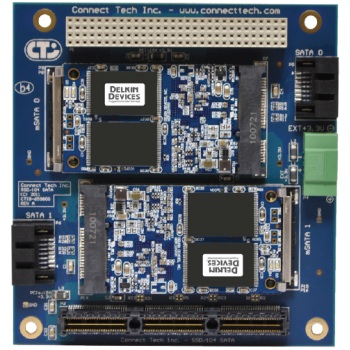
\includegraphics[width=6cm,height=6cm,keepaspectratio]{Pictures/ssd.jpg}
    \caption{SSD Board}
    \label{fig:specs3}
\end{minipage}
\begin{minipage}[b]{0.45\linewidth}
    \centering
    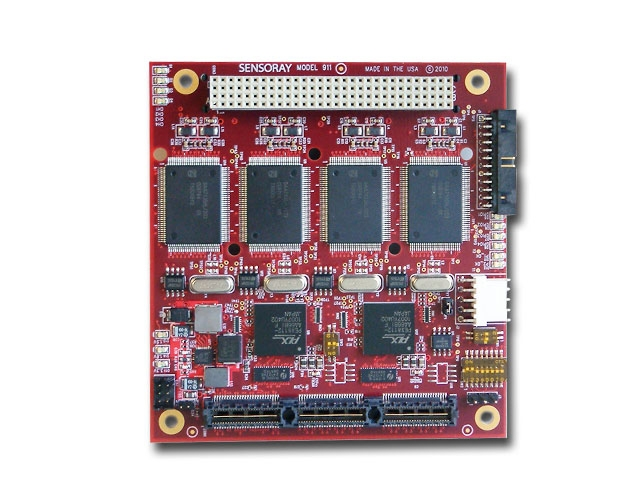
\includegraphics[width=9cm,height=9cm,keepaspectratio]{/Users/KRJ/Dropbox/Research/Latex Thesis Document/Pictures/framegrabber.jpg}
    \caption{Framegrabber}
    \label{fig:specs2}
\end{minipage}
\end{figure}

\subsection{PCI-104 to PC-104 Converter}
This Interface board connects the old PC-104 form factor-based boards to the newer PCI-104 bus. This board is used to interface the older ADC and motor controller with the controller board. The API provided by Connect Tech is useful in interfacing the boards. Figure \ref{fig:specs4} shows a picture of the board.
\begin{figure}[ht]
\begin{minipage}[b]{0.45\linewidth}
    \centering
    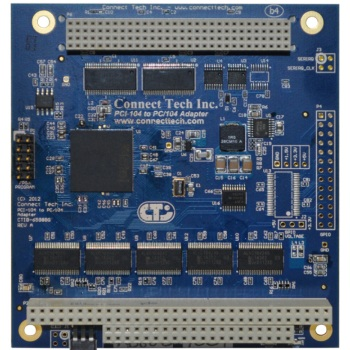
\includegraphics[width=6cm,height=6cm,keepaspectratio]{Pictures/bridge.jpg}
    \caption{ Converter Board}
    \label{fig:specs4}
\end{minipage}
\begin{minipage}[b]{0.45\linewidth}
    \centering
    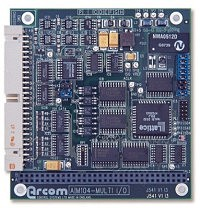
\includegraphics[width=6cm,height=6cm,keepaspectratio]{Pictures/multiIO.jpg}
    \caption{ADC Card}
    \label{fig:specs5}
\end{minipage}
\end{figure}


\subsection{A/D Converter}
AIM104 multi IO is an 8-bit PC-104 module providing 8 Opto-isolated digital inputs and 2 analog outputs, that can be used as 16 single ended inputs or 8 differential inputs. The A/D card is connected to the controller board using the Connect Tech PC-104 to PCI-104 plus adapter. This A/D board is used to connect to the potentiometer, steering motor and accelerometer using interfacing circuits given in \cite{dhake2007real, woodley1999testbed}, Figure \ref{fig:specs5} shows a picture of the board.

\subsection{Motor Controller}
The card used is a 4I27 motor controller card from MESA Electronics with a 7I25 H-Bridge driver to power and operate the motor. It is stacked on the PC-104 bus through the conversion adapter. This is a 2-axis DC servo motor controller that uses a PID filter to set to controller parameters. 4I27 is equipped with two LM629 processors, that can be set to control two separate motors separately without any intervention from the host computer.
The 7I25 needs an external power supply to power the motors. The 7I25 is connected to the main 4I27 board using a 50-pin connector. 

This assembly also consists of an optical shaft encoder, that gives input about the speed of the motor being driven by the H-Bridge driver. The motor feedback can be directly given to the 7I25 H Bridge. Figures \ref{fig:specs6} and \ref{fig:specs7}, show each component separately.

\begin{figure}[ht]
\begin{minipage}[b]{0.45\linewidth}
    \centering
    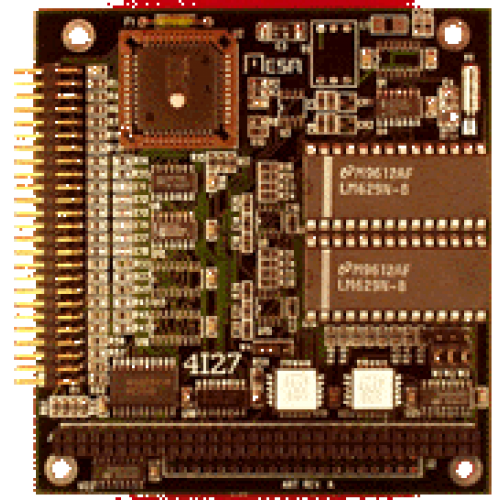
\includegraphics[width=6cm,height=6cm,keepaspectratio]{Pictures/4I27.png}
    \caption{Motor Controller}
    \label{fig:specs6}
\end{minipage}
\begin{minipage}[b]{0.45\linewidth}
    \centering
    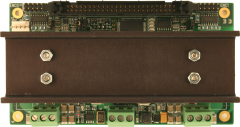
\includegraphics[width=6cm,height=6cm,keepaspectratio]{Pictures/7I25.png}
    \caption{7I25 H-Bridge}
    \label{fig:specs7}
\end{minipage}
\end{figure}
\subsection{Accelerometer}
The accelerometer in the test bed is a Dimension Engineering DE-ACCM3D 3D analog accelerometer. It can measure static and dynamic accelerations. The accelerometer provides x, y and z outputs according to the voltages in the x, y and z directions. The accelerometer is powered by an on board 3.3V voltage source. Figure \ref{fig:specs8} shows a picture of the board as given in \cite{dhake2007real, woodley1999testbed}.

\begin{figure}[ht]
\begin{minipage}[b]{0.45\linewidth}
    \centering
    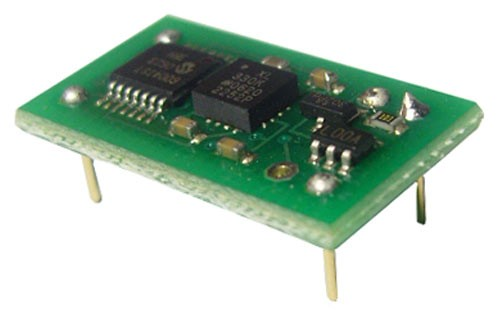
\includegraphics[width=6cm,height=6cm,keepaspectratio]{Pictures/acc.jpg}
    \caption{Accelerometer}
    \label{fig:specs8}
\end{minipage}
\begin{minipage}[b]{0.45\linewidth}
    \centering
    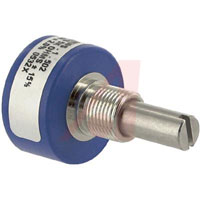
\includegraphics[width=6cm,height=6cm,keepaspectratio]{Pictures/pot.jpg}
    \caption{Potentiometer}
    \label{fig:specs9}
\end{minipage}
\end{figure}

\subsection{Potentiometer}
The test bed vehicle consists of a 50K precision potentiometer from Bourns embedded in the socket between the trailer and the truck. This potentiometer is used to measure the trailer cab angle, which is critical to avoid jackknifing of the truck. Potentiometer uses a 5v DC power supply. Figure \ref{fig:specs9} shows a picture of the potentiometer.


\subsection{Steering Motor}
Steering motor used in this project is a DC servomotor, which has been modified to work with the current configuration as shown in \cite{woodley1999testbed}. The FUTUBA FP-S148 is connected to the ADC from which it gets the signal for steering. Figure \ref{fig:specs10} shows a picture of the steering motor.

\begin{figure}[ht]
\begin{minipage}[b]{0.45\linewidth}
    \centering
    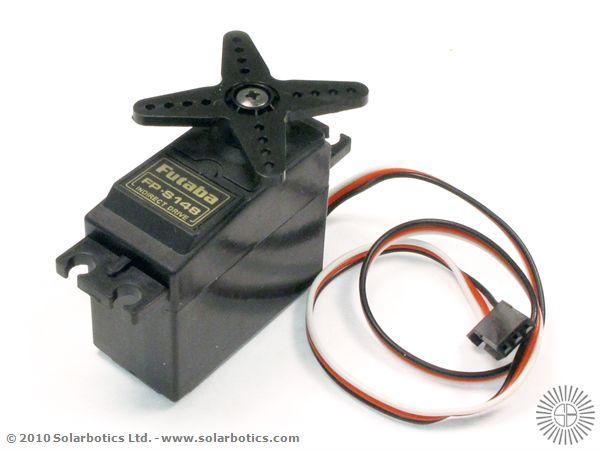
\includegraphics[width=6cm,height=6cm,keepaspectratio]{Pictures/FP.jpg}
    \caption{Steering Motor}
    \label{fig:specs10}
\end{minipage}
\begin{minipage}[b]{0.45\linewidth}
    \centering
    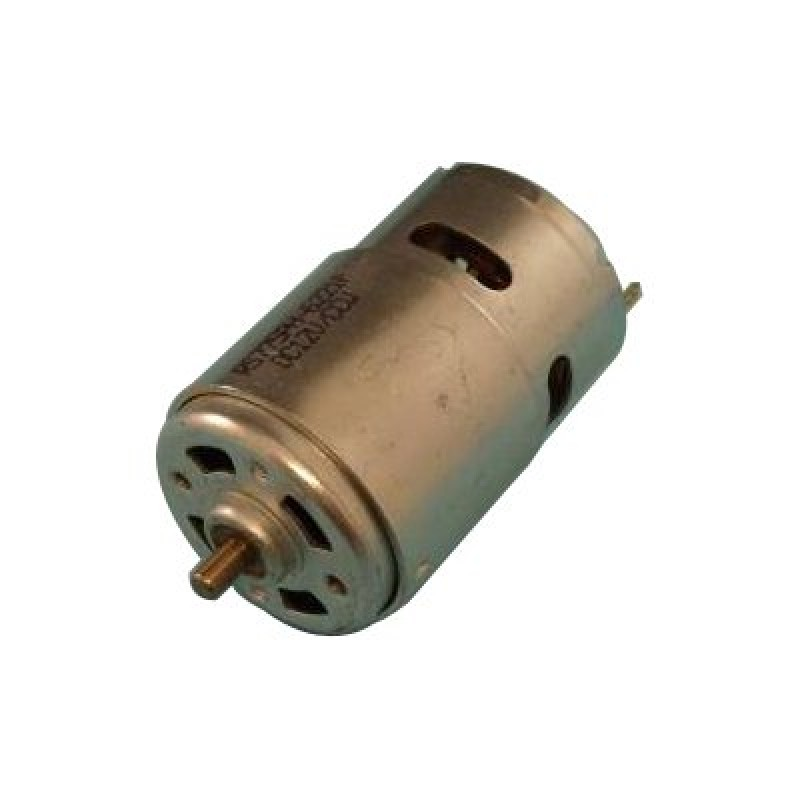
\includegraphics[width=6cm,height=6cm,keepaspectratio]{Pictures/DCMotor.jpg}
    \caption{DC Motor}
    \label{fig:specs11}
\end{minipage}
\end{figure}
\subsection{Driver Motor}
This is a Bane Bots permanent magnet DC brush motor. This motor has an optical shaft encoder connected to it and is controlled using the LM-629 motion controller through the H-bridge driver. The H-Bridge driver supplies power to the motor. Figure \ref{fig:specs11} shows a picture of the driver motor as shown in \cite{dhake2007real,woodley1999testbed}.

\section{Hardware Connectivity}

Table 2.3 provides the partition of the storage memory during the operating system Installation. 
\begin {table}[t]
 \centering
   \caption{Partition of the OS }
 \begin{tabular}{||c|c||}
 \hline \hline
  $\textbf{Partition}$  &   $\textbf{Size}$\\
 \hline \hline
  Swap  & 3 GB \\
 \hline
 Boot  & 250 MB \\
 \hline
 Home    & 20 GB\\
\hline
/    & 56.75 GB\\ 
\hline
Store   & 40GB \\
\hline\hline
 \end{tabular}

\label{table:OSsize}
\end{table}
The Figure \ref{fig:HW} lists the connected components.
\begin{figure}[h]
\centering
    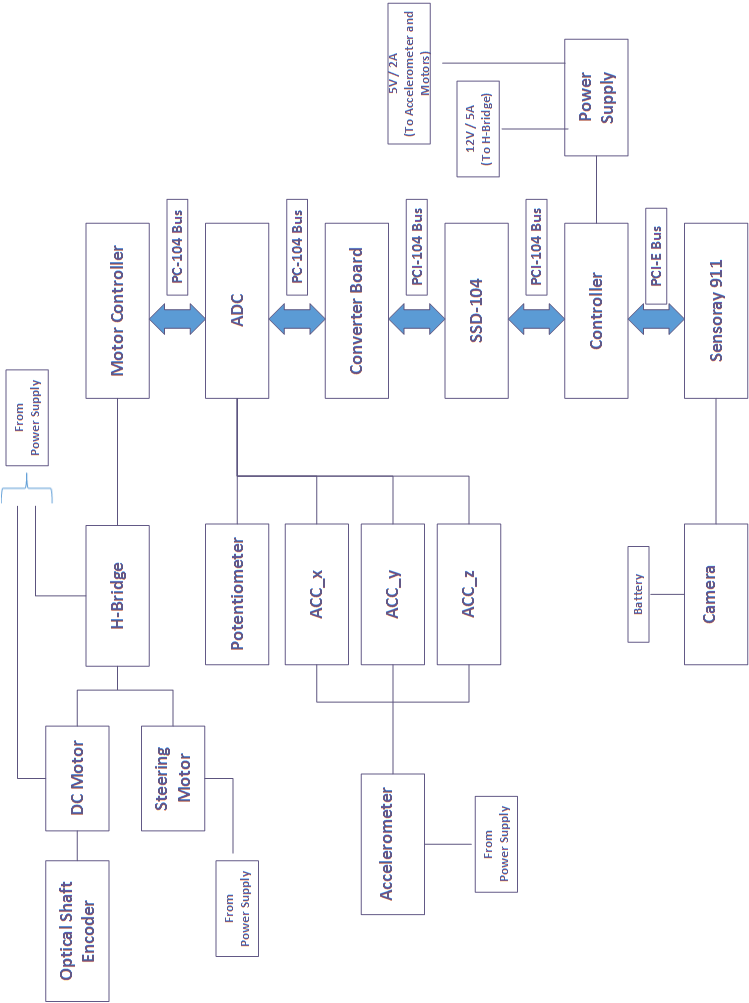
\includegraphics[width=17cm,height=16cm,keepaspectratio]{Pictures/HW_block.png}
    \caption{Block Diagram of the Hardware \label{fig:HW}} 
\end{figure}


\begin {table}[ht]
 \centering
 \caption{Overview of Hardware Update Times \label{table:time}}
 \begin{sideways}
 \begin{tabular}{||p{0.15\textwidth}|p{0.12\textwidth}|p{0.12\textwidth}|p{0.25\textwidth}|p{0.25\textwidth}|p{0.3\textwidth}||}
 \hline \hline
  $\vspace{0.03in} \textbf{Sensors}$ & $\vspace{0.03in} \textbf{Actuators}$ & $\vspace{0.03in}\textbf{Hardware}$ & $\vspace{0.03in} \textbf{Range(Data)/Capacity}$ & $\vspace{0.03in} \textbf{Range(i/p - o/p) }$ & $\textbf{Update Time across Port}$\\
 \hline \hline
Truck Pot &   &  & 12 bits across ADC & i/p - o/p 0-5V & 500 microsecond\\
 \hline
Steering Pot &   &  & 12 bits across ADC & i/p - o/p 0-5V & 500 microsecond\\
 \hline
Shaft Encoder &   &  & Max frequency 200 MHZ & i/p - 5V & 256 microsecond\\
\hline
Accelerometer &   &  & 12 bits across ADC & i/p - o/p 1.33-1.66V & 500 microsecond\\
\hline
 Camera&  &  &130 fps  & 6V & 500 millisecond\\
\hline
 & Steering Motor  &  & & i/p PWM pulses from motor controller & 256 microsecond\\
\hline
& Driving Motor  &  & & i/p PWM pulses from motor controller & 256 microsecond\\
\hline
&   & ADC& -5-5V& 12 bit & 500 microsecond\\
\hline
&   & DAC& -5-5V& 12 bit & 320 microsecond\\
\hline\hline
\end{tabular}
\end{sideways}

\end{table}



